\section{Rendering 3D}
\label{sec:chapter_stato_arte_rendering3d}

Per Rendering si intende il processo di generazione di un’ immagine a due dimensioni a partire una scena, ovvero la definizione matematica di oggetti, materiali, luci ed una camera all’interno di un ambiente a tre dimensioni.
Il Rendering viene utilizzato principalmente nell’ industria videoludica, cinematografica e nell’ architettura; quest’ultimo caso, in particolare, verrà preso in esame per il presente lavoro di tesi.

\begin{figure}[htb]
 \centering
 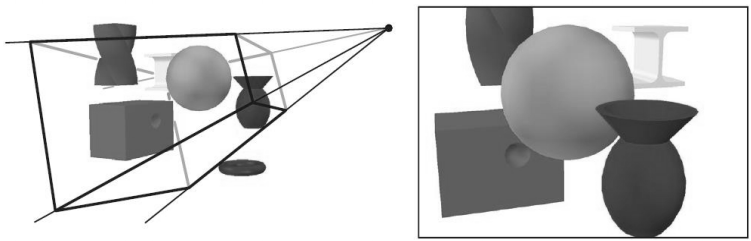
\includegraphics[width=1.0\linewidth]{images/chapter_stato_arte/stato_arte_rendering_3d.png}\hfill
 \caption[Rendering 3D]{Rendering 3D}
 \label{fig:stato_arte_rendering_3d}
\end{figure}

In ambienti grafici 3D è possibile effettutare pre-rendering, o rendering in real-time.

Il rendering real-time, usato principalmente per la creazione di videogiochi in 3D, ha a che fare con la generazione su di un computer di immagini in breve tempo. E’ il processo più interattivo per quanto riguarda la grafica computazionale, perchè ogni immagine rappresentata è il feedback dell’interazione dell’osservatore con l’immagine precedente. Si viene a creare un ciclo di rendering e reazione ad esso, e ciò avviene con una velocità tale per cui l’osservatore non vede le singole immagini, ma un unico processo dinamico. La rapidità con cui le immagini vengono mostrate su schermo è misurata in frame per secondo (FPS): maggiore è l’FPS, minore è il tempo di risposta ad un azione dell’osservatore, migliore è l’interattività. Allo stato attuale, il rendering in real-time è possibile grazie all’esistenza di componenti hardware dedicate all’accelerazione grafica: le unità di processamento grafico, o GPU. Esse sono in grado di gestire, ad ogni frame, milioni se non miliardi di pixels. Tuttavia è importante sottolineare il fatto che il rendering real-time porta a risultati qualitativamente peggiori rispetto ad un rendering off-line (o pre-rendering), anche se il divario tra i due tende ad assottigliarsi.

Il pre-rendering è il processo nel quale le immagini da mostrare non vengono renderizzate in real-time dall’ hardware che riproduce il video, piuttosto esse vengono renderizzate precedentemente da un hardware differente, tipicamente più potente di quello utilizzato, e poi usate durante la riproduzione.
Il processo di fatto permette di diminuire enormemente il carico di lavoro della macchina addetta alla riproduzione video in quanto essa si limita solamente a mostrare immagini pre-calcolate da un’ altra macchina, senza effettuare alcun calcolo di rendering.

